\title{%
  A Science of Security Course, Revisited
}
\author{Daniel Bosk}
\institute{%
  KTH EECS, \email{dbosk@kth.se}
}

\mode<article>{\maketitle}
\mode<presentation>{%
  \begin{frame}
    \maketitle
  \end{frame}
}

\mode*

\begin{abstract}
  \mode*

% What's the problem?
% Why is it a problem? Research gap left by other approaches?
% Why is it important? Why care?
% What's the approach? How to solve the problem?
% What's the findings? How was it evaluated, what are the results, limitations, 
% what remains to be done?

% XXX Summary
\emph{Summary:}
In this learning session we will give an introduction to the scientific method 
and particularly how this can be applied in the area of security.

% XXX Motivation and intended learning outcomes
\emph{Intended learning outcomes:}
After this session you should be able:
\begin{itemize}
  \item to \emph{apply} the scientific method correctly to answer basic 
    questions in security.
\end{itemize}

% XXX Prerequisites
%\emph{Prerequisites:}
%\dots

% XXX Reading material
\emph{Reading:}
You should read 
\citetitle{HowToDesignSecurityExperiments}~\cite{HowToDesignSecurityExperiments}.
This paper discusses the scientific method of (parts of) the security field.
For a more in-depth reflection on the state of security as a scientific pursuit, 
we recommend
\citetitle{SecurityAsAScience}~\cite{SecurityAsAScience}.

\end{abstract}


\section{Overview}

\subsection{Previously on SWITS}

\begin{frame}
  \begin{block}{SWITS 2020}
    \begin{itemize}
      \item Talk: A Science of Security Course
    \end{itemize}
  \end{block}

  \pause

  \begin{block}{The goal}
    \begin{itemize}
      \item Give a holistic view of Science of Security.
      \item What are the methods we use and why?
      \item Where are the disputes, philosophical problems and why?
    \end{itemize}
  \end{block}
\end{frame}

\begin{frame}
  \fullcite{SecurityAsAScience}
\end{frame}

\begin{frame}[fragile]
  \begin{example}
      \textcquote[\S IV]{SecurityAsAScience}{\textins*{C}laims of necessary 
        conditions for real-world security are unfalsifiable.
      Claims of necessary conditions for formally-defined security are 
    tautological restatements of the assumptions}.
  \end{example}

  \pause

  \begin{example}
    \textcquote{SecurityAsAScience}{%
      Unfalsifiable claims are common in security---and they, along with circular 
      arguments, are used to justify many defensive measures \textelp{}
      \textins{T}here are many ways to argue measures in, but no way to argue one 
      out.
    }
  \end{example}
\end{frame}

\begin{frame}
  \begin{question}
    \begin{itemize}
      \item What makes my work scientific?
    \end{itemize}
  \end{question}
\end{frame}

\subsection{A master's programme}

\begin{frame}[fragile]
  \begin{block}{MSc Cybersecurity}
    \begin{description}
      \item[Programme co-ordinators] Sonja Buchegger and Mathias Ekstedt
      \item[Started] Autumn 2022
      \item[First round of theses] Spring 2024
    \end{description}
  \end{block}
\end{frame}

\begin{frame}
  \begin{remark}
    \begin{itemize}
      \item My previous experience of master students is that their skills 
        leave some things to be desired.
    \end{itemize}
  \end{remark}

  \pause

  \begin{block}{Aim of Science of Security course}
    \begin{itemize}
      \item Complement the general methods course.
      \item Better prepare students for thesis (and hopefully worklife \dots).
      \item They should be able to contribute to scientifically based 
        development in cybersecurity.
    \end{itemize}
  \end{block}
\end{frame}

\begin{frame}[fragile]
  After passing the course, the student should be able to
  \begin{itemize}
    \item<+> relate the different parts of scientific method, how they relate 
      to one another, contribute and not contribute to scientificity in 
      security
    \item<+> assess, analyse, and discuss the quality in, and ethical aspects 
      of, knowledge generation related to digital systems and in particular the 
      security of these systems
    \item<+> apply scientific methodology to show how to answer issues in the 
      cybersecurity field
    \item<+> \dots
%    \item<+> plan and carry out assignments within given time frames and 
%      available resources
%    \item<+> write short, clear and arguing texts based on own analysis as well 
%      as given material.
  \end{itemize}
  in order to be able to contribute to scientifically based development.
\end{frame}

\begin{frame}[fragile]
  \footnotesize
  \begin{columns}[t]
    \begin{column}{0.5\columnwidth}
      \begin{block}{Master's goals~\cite{HEO2}}
        \begin{itemize}
          \item demonstrate knowledge and understanding \textelp{} as well as 
            insight into current research and development work, and
          \item demonstrate specialised methodological knowledge in the main 
            field of study.
          \item demonstrate the ability to critically and systematically 
            integrate knowledge and analyse, assess and deal with complex 
            phenomena, issues and situations even with limited information
        \end{itemize}
      \end{block}
    \end{column}
    \begin{column}{0.5\columnwidth}
      \begin{block}{PhD goals~\cite{HEO2}}
        \begin{itemize}
          \item demonstrate familiarity with research methodology in general 
            and the methods of the specific field of research in particular.
          \item demonstrate the capacity for scholarly analysis and synthesis as 
            well as to review and assess new and complex phenomena, issues and 
            situations autonomously and critically
        \end{itemize}
      \end{block}
    \end{column}
  \end{columns}
\end{frame}

\begin{frame}[fragile]
  \footnotesize
  \begin{columns}[t]
    \begin{column}{0.5\columnwidth}
      \begin{block}{Master's goals~\cite{HEO2}}
        \begin{itemize}
          \item demonstrate the ability to identify and formulate issues 
            critically, autonomously and creatively as well as to plan and, 
            using appropriate methods, undertake advanced tasks \textelp{} and 
            so contribute to the formation of knowledge as well as the ability 
            to evaluate this work
          \item demonstrate the ability \textelp{} to plan and, using 
            appropriate methods, undertake advanced tasks \textelp{} and so 
            contribute to the formation of knowledge as well as the ability to 
            evaluate this work
          \item demonstrate the skills required for participation in research
            \textelp{}
            %and development work \textelp{}
        \end{itemize}
      \end{block}
    \end{column}
    \begin{column}{0.5\columnwidth}
      \begin{block}{PhD goals~\cite{HEO2}}
        \begin{itemize}
          \item demonstrate the ability to identify and formulate issues with 
            scholarly precision critically, autonomously and creatively, and to 
            plan and use appropriate methods to undertake research and other 
            qualified tasks within predetermined time frames and to review and 
            evaluate such work
        \end{itemize}
      \end{block}
    \end{column}
  \end{columns}
\end{frame}

\begin{frame}[fragile]
  \footnotesize
  \begin{columns}[t]
    \begin{column}{0.5\columnwidth}
      \begin{block}{Master's goals~\cite{HEO2}}
        \begin{itemize}
          \item demonstrate the ability to make assessments in the main field 
            of study informed by relevant disciplinary, social and ethical 
            issues and also to demonstrate awareness of ethical aspects of 
            research and development work
          \item demonstrate insight into the possibilities and limitations of 
            research, \textelp{}
        \end{itemize}
      \end{block}
    \end{column}
    \begin{column}{0.5\columnwidth}
      \begin{block}{PhD goals~\cite{HEO2}}
        \begin{itemize}
          \item demonstrate intellectual autonomy and disciplinary rectitude as 
            well as the ability to make assessments of research ethics, and
          \item demonstrate specialised insight into the possibilities and 
            limitations of research, its role in society and the responsibility 
            of the individual for how it is used.
        \end{itemize}
      \end{block}
    \end{column}
  \end{columns}
\end{frame}

\begin{frame}[fragile]
  \begin{block}{Conclusion goals}
    \begin{itemize}
      \item The goals are very similar.
      \item It's \enquote{just} a matter of progression.
    \end{itemize}
  \end{block}

  \begin{remark}
    \begin{itemize}
      \item Even not adapted to PhD students, it would be a boost towards the 
        goals of the PhD degree.
      \item (Based on the 2020 discussion.)
    \end{itemize}
  \end{remark}
\end{frame}


\section{More concretely}

\subsection{The goal}

\begin{frame}
  \begin{example}[\enquote{Provable security}]
    \begin{itemize}
      \item A uniformly random string of length \(n\) is the most secure 
        password.

      \item We can prove it will take millions of years to guess it.
    \end{itemize}
  \end{example}

  \pause

  \begin{remark}
    \begin{itemize}
      \item Attackers still get in, weird \dots
    \end{itemize}
  \end{remark}
\end{frame}

\begin{frame}
  \begin{example}[Usability]
    \begin{itemize}
      \item Turns out people can't handle uniformly random passwords.
      \item Particularly not with a unique such password for every service.
      \item They can't generate uniformly random passwords either.
    \end{itemize}
  \end{example}

  \pause

  \begin{remark}[Several aspects]
    \begin{itemize}
      \item We want students to handle complex problems.
      \item Should see there are several aspects.
      \item Aspects must be approached differently.
    \end{itemize}
  \end{remark}
\end{frame}


\subsection{Contents}

\begin{frame}
  \begin{block}{Contents}
    \begin{itemize}
      \item Overview of the complexity
    \end{itemize}
    \begin{enumerate}
      \item Purely deductive methods
      \item[\vdots]
      \item[n] Purely inductive methods
    \end{enumerate}
    \begin{itemize}
      \item {Philosophy of Science of Security}
    \end{itemize}
  \end{block}

  \pause

  \begin{remark}[What to focus]
    \begin{itemize}
      \item What does the method contribute?
      \item How do these play together? (Holistic view)
      %\item Emphasize the deduction/induction 
        %divide~\cite{SecurityAsAScience}.
    \end{itemize}
  \end{remark}
\end{frame}

\begin{frame}
  \begin{example}[Deductive inquiry]
    \begin{itemize}
      \item \enquote{What can deduction possibly say about reality?}
    \end{itemize}
  \end{example}

  \pause

  \begin{example}[Inductive/empirical inquiry]
    \begin{itemize}
      \item \enquote{What can induction possibly say about security?}
    \end{itemize}
  \end{example}

  \pause

  \begin{remark}[To focus on]
    \begin{itemize}
      \item What are the limitations?
      \item Do these require a combination to form a Science of Security?
    \end{itemize}
  \end{remark}
\end{frame}

\begin{frame}
  \begin{example}[Philosophy of Science of Security]
    \begin{itemize}
      \item Discuss 
        \citetitle{SecurityAsAScience}\footfullcite{SecurityAsAScience}.
      \item What is Science of Security?
      \item Does that even exist at the moment?
      \item Shall we work according to the hypothetico-deductive model?
      \item What are the problems?
    \end{itemize}
  \end{example}
\end{frame}

\begin{frame}[fragile]
  \begin{block}{Teaching design}
    \begin{itemize}
      \item Have problems that must be explored using several 
        methods.
      \item Work through enough problems to cover the entire spectrum.
    \end{itemize}
  \end{block}

  \begin{remark}[Learning theory]
    \begin{columns}[T]
      \begin{column}{0.6\columnwidth}
          \centering
          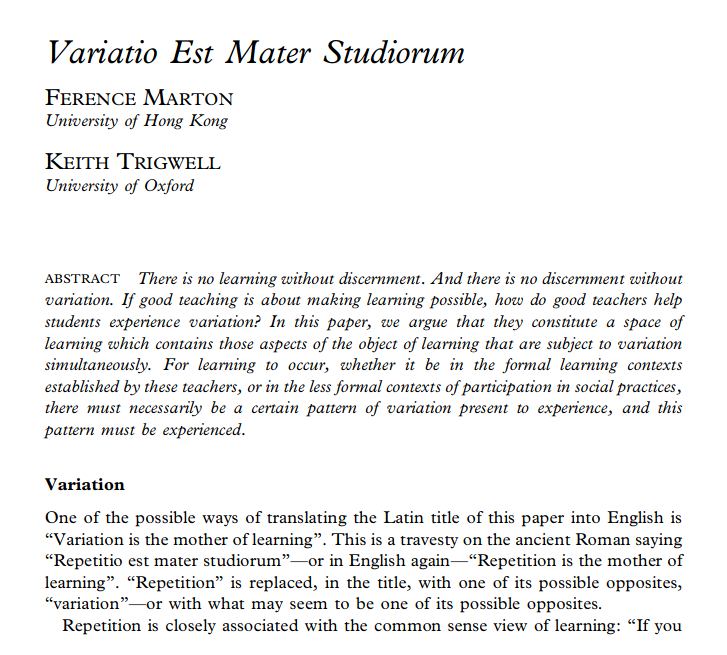
\includegraphics[width=0.8\columnwidth]{figs/variatio-mater-studiorum.png}
        \end{column}
        \begin{column}{0.4\columnwidth}
          
\includegraphics[height=0.55\textheight]{figs/NCOL.jpg}
        \end{column}
      \end{columns}
  \end{remark}
\end{frame}

%\begin{frame}
%  \begin{block}{Contents, part II}
%    \begin{itemize}
%      \item General introductions to various subfields.
%      \item Which methods are used and why?
%      \item Some exemplary papers? \alert<2>{Both good and bad!}
%      \item How does a subfield fit into the holistic picture of Security?
%    \end{itemize}
%  \end{block}
%\end{frame}
%
%\begin{frame}
%  \begin{remark}
%    \begin{itemize}
%      \item All above was top down: faculty\footnote{%
%          From different subfields.
%        } present their view on
%        \begin{itemize}
%          \item the methodologies,
%          \item the practices,
%          \item the adversary models,
%          \item the assumptions,
%          \item the relation to scientific approach in their respective 
%            subfield.
%        \end{itemize}
%    \end{itemize}
%  \end{remark}
%\end{frame}
%
%\begin{frame}
%  \begin{block}{Bottom up}
%    \begin{itemize}
%      \item Course participants review the scientific merits of 
%        papers\footnote{%
%          Chosen by subfield designer, not participants.
%        } from top conferences in the subfield.
%
%      \item They identify/reverse engineer methodology and components of 
%        evaluation.
%
%      \item They value why this is scientific and how and what knowledge it 
%        contributes.
%    \end{itemize}
%  \end{block}
%\end{frame}
%
%\begin{frame}[allowframebreaks]
%  \begin{block}{Assessment}
%    \begin{itemize}
%      \item Apply subfield methodology insights to own paper.
%
%      \item Reflect on how this paper fits in the big picture of Security as a 
%        Science.
%
%      \item Discussion/reflection on limits of how scientific security research 
%        can be; \eg provability versus complexity of actual systems, 
%        engineering versus science.
%
%      \item Peer-review (among course participants) these individual 
%        papers\footnote{%
%          Or a paper in progress or already published paper.
%        } to identify gaps in the scientific approach that could be filled.
%    \end{itemize}
%  \end{block}
%\end{frame}

\subsection{Format}

\begin{frame}[fragile]
  \begin{block}{Examination}
    \begin{description}
      \item[INL1] Seminars and assignments, 3.0 credits, grading scale: P, F
    \end{description}
  \end{block}

  \pause

  \begin{block}{Format}
    \begin{itemize}
      \item Online assignments
      \item Asynchronous, social annotation
      \item One in-place\footnote{%
          For the campus students.
        } final seminar
    \end{itemize}
  \end{block}
\end{frame}

\begin{frame}
  \begin{columns}
    \begin{column}{0.5\columnwidth}
      \begin{block}{Teaching material}
        \begin{itemize}
          \item<1> Video lectures where students can ask questions and answer 
            quizzes\footnote{FeedbackFruits or Canvas Studio}.

            \pause

          \item<2-3> Reading assignments with social annotation\footnote{%
              FeedbackFruits or Perusall
            }.
        \end{itemize}
      \end{block}
    \end{column}
    \begin{column}{0.5\columnwidth}
      \begin{figure}
        \centering
        \only<1>{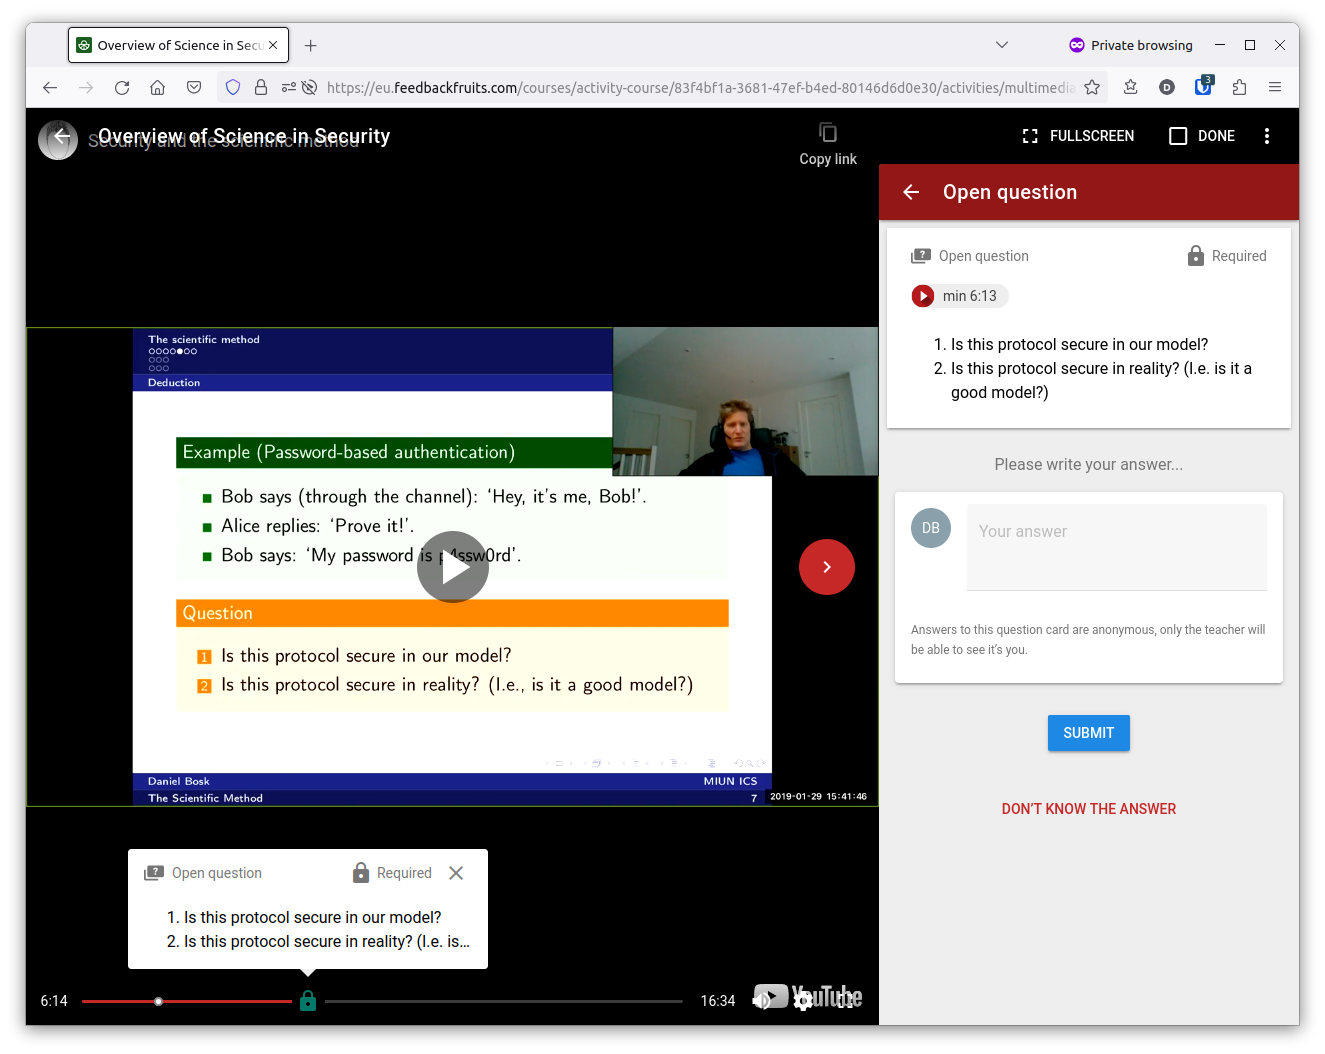
\includegraphics[width=\columnwidth]{figs/fbf-video-quiz.png}}
        \only<3>{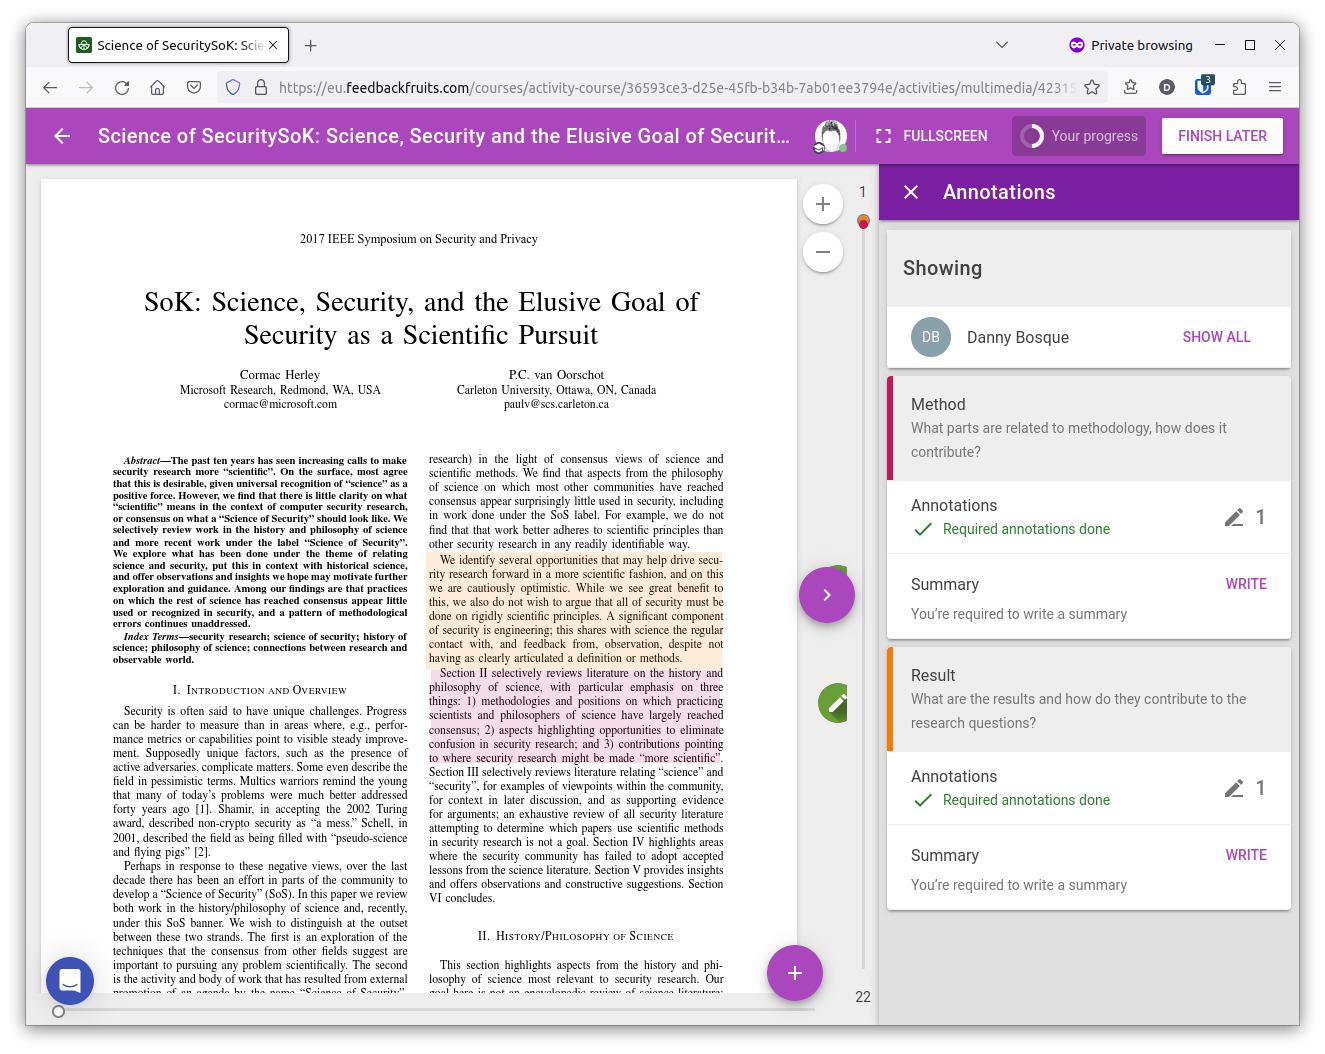
\includegraphics[width=\columnwidth]{figs/fbf-doc-annotations.png}}
        \only<2>{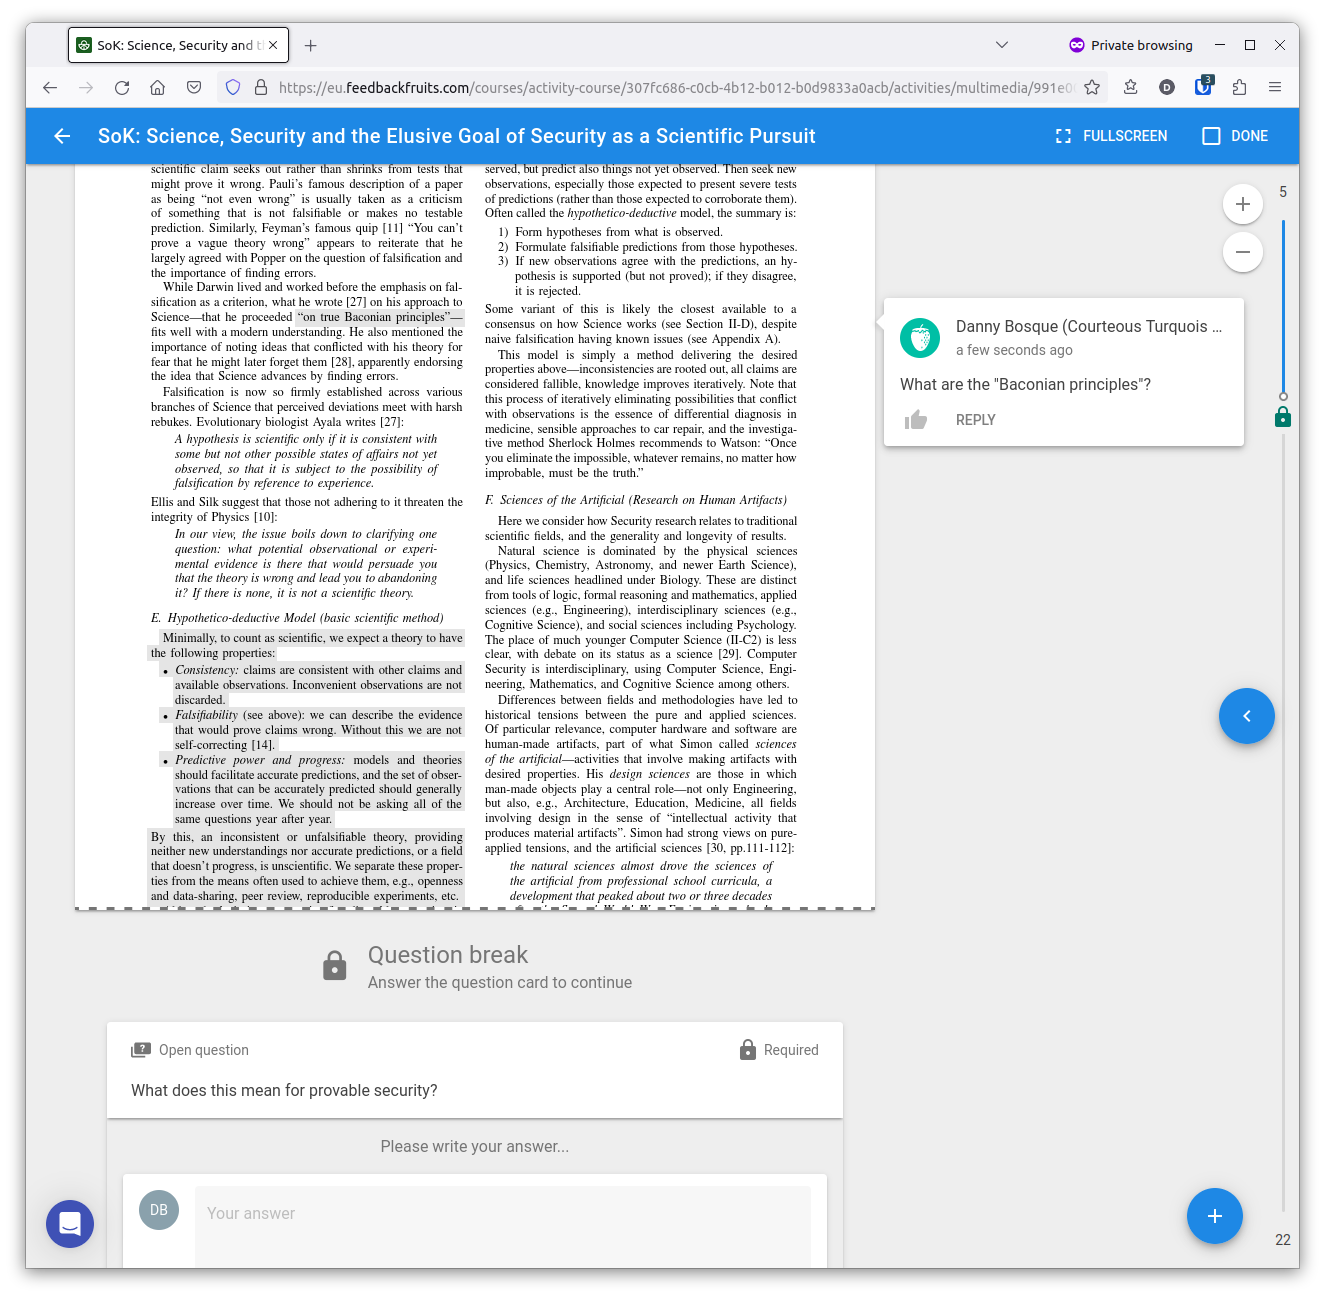
\includegraphics[width=\columnwidth]{figs/fbf-doc-quiz-question.png}}
      \end{figure}
    \end{column}
  \end{columns}
\end{frame}

\begin{frame}
  \begin{block}{Assessment}
    \begin{itemize}
      \item A synchronous seminar to summarize all work and tie the sack.
    \end{itemize}
  \end{block}
\end{frame}

\begin{frame}
  \begin{block}{Giving the course}
    \begin{enumerate}
      \item Given every period; yes, four times per year.
    \end{enumerate}
  \end{block}

  \pause

  \begin{remark}
    \begin{enumerate}
      \item Asynchronicity and frequency are good for PhD students.
      \item Joint with master's is good for funding it.
    \end{enumerate}
  \end{remark}
\end{frame}


\section{Conclusions and discussion}

\begin{frame}
  \begin{block}{From 2020}
    \begin{itemize}
      \item<+> Emphasis on practice, not only on philosophy of science, to be 
        able to evaluate how strong a claim is justified in one's own and 
        others' publications and to learn to apply scientific methods to 
        increase the confidence in new results.

      \item<+> How is the progression compared to the \enquote{normal} 
        methodology  course?
        \begin{itemize}
          \item What is the added value?
          \item Focus on specifics of security, assume participants have taken 
            \enquote{regular} research methods course.
        \end{itemize}

      \item<+> Target audience? Half-way-through students?

      \item<+> 20+ students said they wanted such a course.
    \end{itemize}
  \end{block}
\end{frame}

\begin{frame}[fragile]
  \begin{columns}
    \begin{column}{0.7\columnwidth}
      \begin{block}{Available on GitHub}
        \begin{itemize}
          \item \url{https://github.com/OpenSecEd/scientific-method}
        \end{itemize}
      \end{block}
    \end{column}
    \begin{column}{0.3\columnwidth}
      
\includegraphics[width=\columnwidth]{figs/GHurl.png}
    \end{column}
  \end{columns}

  \begin{remark}[Contributions]
    \begin{itemize}
      \item Good \emph{and bad} work!
      \item Literature on methods in security
      \item Videos if you want to talk about your favourite methods.
      \item Just add thoughts to issue tracker on GH.
    \end{itemize}
  \end{remark}
\end{frame}

\begin{frame}
  \begin{question}
    \begin{itemize}
      \item Comments, questions, other thoughts?
    \end{itemize}
  \end{question}
\end{frame}


%%% REFERENCES %%%

\begin{frame}[allowframebreaks]
  \printbibliography
\end{frame}

